% Options for packages loaded elsewhere
\PassOptionsToPackage{unicode}{hyperref}
\PassOptionsToPackage{hyphens}{url}
\PassOptionsToPackage{space}{xeCJK}
\documentclass[
  chinese,
]{article}
\usepackage{xcolor}
\usepackage{amsmath,amssymb}
\setcounter{secnumdepth}{-\maxdimen} % remove section numbering
\usepackage{iftex}
\ifPDFTeX
  \usepackage[T1]{fontenc}
  \usepackage[utf8]{inputenc}
  \usepackage{textcomp} % provide euro and other symbols
\else % if luatex or xetex
  \usepackage{unicode-math} % this also loads fontspec
  \defaultfontfeatures{Scale=MatchLowercase}
  \defaultfontfeatures[\rmfamily]{Ligatures=TeX,Scale=1}
\fi
\usepackage{lmodern}
\ifPDFTeX\else
  % xetex/luatex font selection
  \ifXeTeX
    \usepackage{xeCJK}
    \setCJKmainfont[]{Microsoft YaHei}
    \setCJKsansfont[]{Microsoft YaHei}
    \setCJKmonofont[]{Microsoft YaHei}
  \fi
  \ifLuaTeX
    \usepackage[]{luatexja-fontspec}
    \setmainjfont[]{Microsoft YaHei}
  \fi
\fi
% Use upquote if available, for straight quotes in verbatim environments
\IfFileExists{upquote.sty}{\usepackage{upquote}}{}
\IfFileExists{microtype.sty}{% use microtype if available
  \usepackage[]{microtype}
  \UseMicrotypeSet[protrusion]{basicmath} % disable protrusion for tt fonts
}{}
\makeatletter
\@ifundefined{KOMAClassName}{% if non-KOMA class
  \IfFileExists{parskip.sty}{%
    \usepackage{parskip}
  }{% else
    \setlength{\parindent}{0pt}
    \setlength{\parskip}{6pt plus 2pt minus 1pt}}
}{% if KOMA class
  \KOMAoptions{parskip=half}}
\makeatother
\usepackage{longtable,booktabs,array}
\usepackage{calc} % for calculating minipage widths
% Correct order of tables after \paragraph or \subparagraph
\usepackage{etoolbox}
\makeatletter
\patchcmd\longtable{\par}{\if@noskipsec\mbox{}\fi\par}{}{}
\makeatother
% Allow footnotes in longtable head/foot
\IfFileExists{footnotehyper.sty}{\usepackage{footnotehyper}}{\usepackage{footnote}}
\makesavenoteenv{longtable}
\usepackage{graphicx}
\makeatletter
\newsavebox\pandoc@box
\newcommand*\pandocbounded[1]{% scales image to fit in text height/width
  \sbox\pandoc@box{#1}%
  \Gscale@div\@tempa{\textheight}{\dimexpr\ht\pandoc@box+\dp\pandoc@box\relax}%
  \Gscale@div\@tempb{\linewidth}{\wd\pandoc@box}%
  \ifdim\@tempb\p@<\@tempa\p@\let\@tempa\@tempb\fi% select the smaller of both
  \ifdim\@tempa\p@<\p@\scalebox{\@tempa}{\usebox\pandoc@box}%
  \else\usebox{\pandoc@box}%
  \fi%
}
% Set default figure placement to htbp
\def\fps@figure{htbp}
\makeatother
\ifLuaTeX
\usepackage[bidi=basic,shorthands=off,,provide=*]{babel}
\else
\usepackage[bidi=default,shorthands=off,,provide=*]{babel}
\fi
\ifLuaTeX
  \usepackage{selnolig} % disable illegal ligatures
\fi
\setlength{\emergencystretch}{3em} % prevent overfull lines
\providecommand{\tightlist}{%
  \setlength{\itemsep}{0pt}\setlength{\parskip}{0pt}}
\usepackage{bookmark}
\IfFileExists{xurl.sty}{\usepackage{xurl}}{} % add URL line breaks if available
\urlstyle{same}
\hypersetup{
  pdftitle={高效视觉 Transformer 的方法学图谱（2021--2026）：证据约束小型综述},
  pdflang={zh-CN},
  hidelinks,
  pdfcreator={LaTeX via pandoc}}

\title{高效视觉 Transformer
的方法学图谱（2021--2026）：证据约束小型综述}
\usepackage{etoolbox}
\makeatletter
\providecommand{\subtitle}[1]{% add subtitle to \maketitle
  \apptocmd{\@title}{\par {\large #1 \par}}{}{}
}
\makeatother
\subtitle{架构演练稿（spine-001）}
\author{}
\date{}

\begin{document}
\maketitle

\section{摘要}\label{ux6458ux8981}

视觉 Transformer
以自注意力替代卷积，但二次复杂度与显存访问开销限制了其在移动端与
边缘设备上的部署。本文以满足严格计算预算的视觉 Transformer
方法为对象，对 2021--2026 年间经检索层获得的 24
条公开记录做文献层梳理，提出以\textbf{效率来源}为轴的四族分类
（注意力稀疏化、分组与级联、混合
CNN-Transformer、参数共享与模块重构），并给出可判定
样本的\textbf{证据强度分级}。分析显示：在 6
条带摘要记录中，给出参数量数值的 3 条、给出算力 数值的 1
条、给出精度数值的 3 条（三类字段可重叠），而\textbf{同时给出三项者为 0
条}；其余 18 条
仅具元数据而无摘要可供判定。这说明\textbf{跨论文性能比较在本证据基础上不成立}。本文贡献限于文献组织方式
与证据边界的显式化，不含任何新方法或新读数。

\textbf{关键词}：视觉 Transformer；计算效率；轻量化；证据边界；文献组织

\section{1 引言}\label{ux5f15ux8a00}

自注意力在视觉任务上的优势已被广泛接受，但其代价同样明确：注意力计算随
token 数呈
二次增长，且内存访问模式不友好。围绕''如何把成本压下来''，近五年出现了大量改进工作
（R01--R24）。

现有综述多\textbf{按任务分类}（分类、检测、分割、复原、视频），这种组织方式便于按应用检索，
却掩盖了一个更实质的差异：不同方法降低成本的\textbf{来源}并不相同。有的是把注意力范围
限制住（R02、R07），有的是改变通道组织以优化内存访问（R01），有的是让卷积承担局部
建模、注意力专注全局（R10、R13、R14），还有的是靠参数共享或模块重构直接压缩模型
（R03、R16、R17）。把''分类网络''\,``检测网络''和''轻量网络''并列，读者难以判断某项改进到
底缓解了哪一类瓶颈。

本文因此改以\textbf{效率来源}为分类轴，并在同一批文献上额外记录\textbf{指标披露完备度}。后者
不是附带统计，而是理解该领域进展的前提：当多数工作不同时报告参数量、算力与精度时，
任何''谁更高效''的横向判断都缺乏共同基准。

\section{2 方法与范围}\label{ux65b9ux6cd5ux4e0eux8303ux56f4}

\textbf{检索}：经学术检索层（CrossRef / arXiv）以''高效视觉 Transformer
/ 轻量化注意力'' 为主题检索，返回 29 条记录，纳入 24 条。

\textbf{纳入口径}：记录含可核验 DOI 或 arXiv ID，且主题落在视觉
Transformer 的\textbf{计算效率} 改进上。剔除仅涉及 Transformer
一般应用而与效率无关者。\textbf{范围边界}：本批记录中 含 3D
点云（R02）、视频识别（R19、R20）与骨架动作识别（R21）各一支，本文将其一并
纳入''视觉''范畴，并在第 3
节对其是否适用于静态图像分类单独标注，不作默认推广。
\textbf{载体分级标准}：同行评审状态不可确认者（预印本平台，或未被主流索引收录且作者与出版
信息单薄的期刊）记为高风险载体；该标签为\textbf{判断}，不是对论文质量的裁决。本批按此标准
命中 R22、R23（SSRN 预印本）与 R24（未被主流索引收录的期刊）。

\textbf{研究模式}：本任务在 \texttt{materials\_only}
模式下完成，即\textbf{仅使用已发表记录的表层信息}，
不进行任何实验、训练、评测或复现。这一限制直接决定了本文的证据上界：对未提供摘要的
18 条记录，其具体读数\textbf{不可知}。

\textbf{明确的证据边界}（本节的自我约束）：

\begin{enumerate}
\def\labelenumi{\arabic{enumi}.}
\tightlist
\item
  本文\textbf{未获取任何全文 PDF}，未经逐段核对；
\item
  因此第 3
  节的''四族分类''属\textbf{基于标题与摘要的初步归类}，是推断而非论文原文主张；
\item
  本文\textbf{不进行任何跨论文数值比较}，理由见第 4 节。
\end{enumerate}

\section{3 方法族图谱}\label{ux65b9ux6cd5ux65cfux56feux8c31}

按效率来源划分，纳入文献可分为四族：

\textbf{F1 注意力稀疏化与结构化。}
通过限制每个查询可见的区域或引入可微锚点来削减注意力
计算量。代表：PatchFormer 以 patch attention
替代全局注意力（R02）；AnchorFormer 引入 可微锚点注意力（R07）。

\textbf{F2 分组与级联注意力。}
不减少注意力覆盖范围，而是重组通道与计算顺序以改善内存
访问效率。代表：EfficientViT
的级联分组注意力（R01）。这类工作提示：瓶颈未必是浮点
运算量本身，也可能是访存。

\textbf{F3 混合 CNN-Transformer。}
让卷积承担局部特征、注意力承担全局关系，从而在同等
预算下取得折中。代表：MobileNetv1-ViT
混合结构（R13）、LightFER（R14）、面向嵌入式
证件识别的超轻量卷积注意力网络（R10）、MCANet（R06）。

\textbf{F4 参数共享与模块重构。}
通过递归共享参数（R03）、统一的内在残差元模块（R16）或
直接设计亚百万参数档架构（R17）压缩规模。

此外还有两支不属于上述四族：以相对位置编码替代稠密算子（R20），以及冻结大型预训练
骨干、仅训练轻量头部（R19）。二者出现于视频识别与视觉-语言场景，是否适用于静态图像
分类尚不可从现有记录判断。

骨架动作识别一支（R21）以多分类器共识组织轻量系统，其效率来源与上述四族及两支均不可
直接对应，故本演练不为其指定族别，仅保留于纳入范围以备复核。

需要强调：\textbf{该分类是本文提出的组织方式}，而非对原文献主张的复述。

\section{4 证据景观}\label{ux8bc1ux636eux666fux89c2}

图 1 由纳入的 24 条记录的真实元数据计算得到。

\begin{figure}
\centering
\pandocbounded{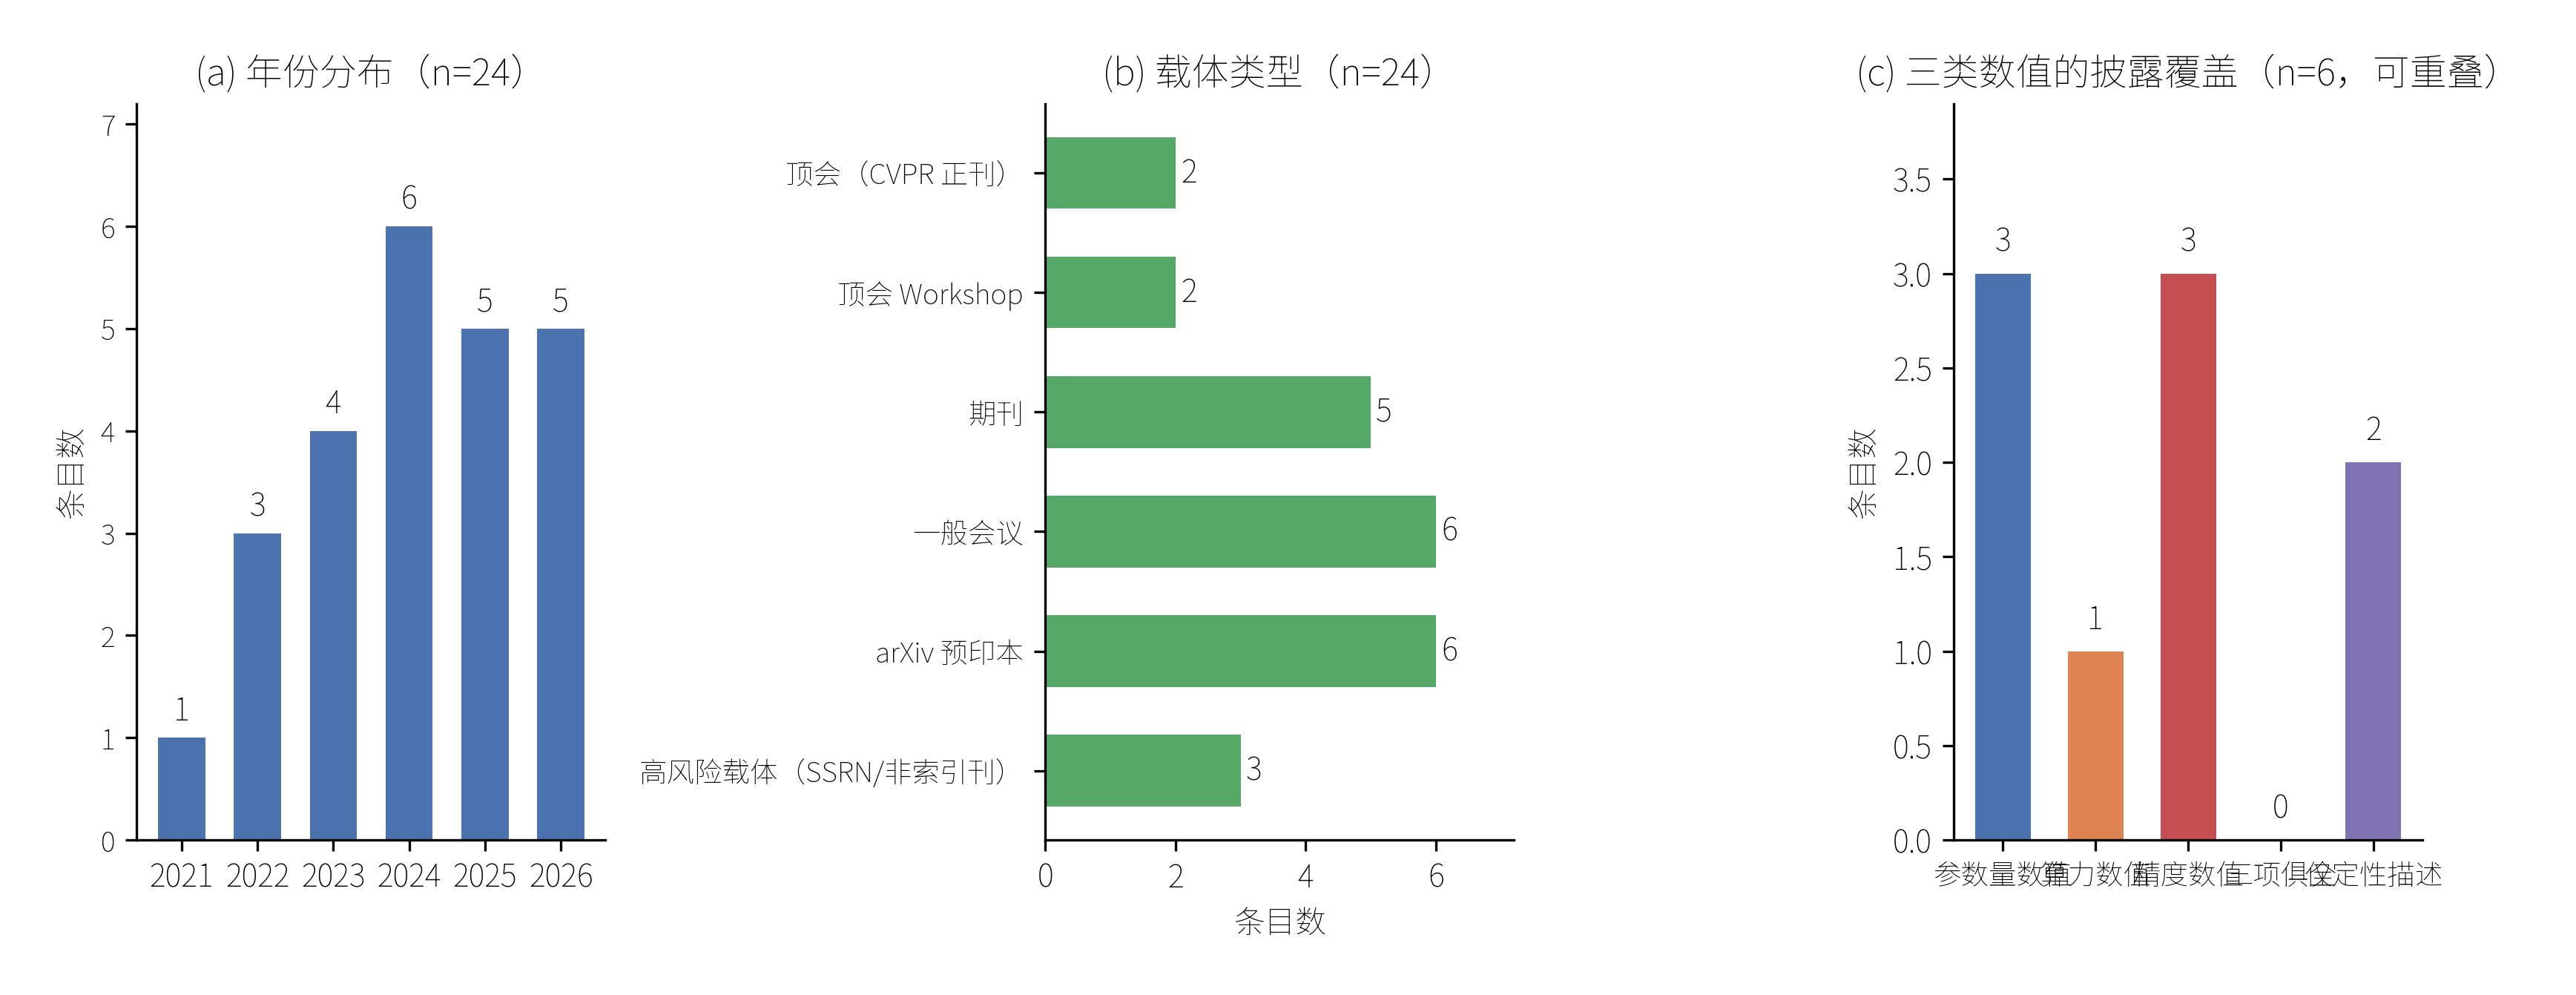
\includegraphics[keepaspectratio,alt={图 1 纳入文献的证据景观。}]{figures/fig1_evidence_landscape.png}}
\caption{图 1 纳入文献的证据景观。}\label{fig:evidence-landscape}
\end{figure}

\textbf{图 1}　纳入文献的证据景观（n = 24）。(a) 年份分布；(b)
载体类型构成；(c) 6 条带摘要 记录中三类数值的披露覆盖（可重叠）。(a)(b)
两项计数可由 \texttt{reference\_materials/source\_index.md}
逐条回算（其中 sci-q1/q2/q3 合并计为期刊，conf 与 spie
合并计为一般会议）； (c) 的逐条依据见 \texttt{evidence\_bank.md} 的 E-A
台账。

三点观察：

\textbf{其一，方向活跃且产出分散。} 年份分布自 2021 年起持续，2024
年达到 6 条。载体构成 中，顶会正刊仅 2 条，Workshop 2 条、期刊 5
条、一般会议 6 条、arXiv 预印本 6 条， 另有 3 条属高风险载体（SSRN
预印本与非索引刊）。\textbf{这一构成意味着：若仅保留顶会正刊
与期刊（本批共 7 条），可用记录将缩减至不足三分之一。}

\textbf{其二，在有摘要子集内评测口径分裂，横向比较不成立。} 在 24
条记录中，可判定披露 情况的只有 6 条（其余 18
条检索层未返回摘要）：其中给出参数量数值的 3 条、给出算力 数值的 1
条、给出精度数值的 3 条，\textbf{同时给出三项者为 0 条}，另有 2
条未给任何数值。由于训练配方、数据划分与评测协议各不相同，\textbf{即使都给出
Top-1， 也不构成可比较的基准}。本文因此不做任何排序或''最优方法''判断。

\textbf{证据强度分级（本批，仅限 6 条带摘要记录）}：

\begin{longtable}[]{@{}
  >{\raggedright\arraybackslash}p{(\linewidth - 4\tabcolsep) * \real{0.3333}}
  >{\raggedright\arraybackslash}p{(\linewidth - 4\tabcolsep) * \real{0.3333}}
  >{\raggedright\arraybackslash}p{(\linewidth - 4\tabcolsep) * \real{0.3333}}@{}}
\toprule\noalign{}
\begin{minipage}[b]{\linewidth}\raggedright
级别
\end{minipage} & \begin{minipage}[b]{\linewidth}\raggedright
判据
\end{minipage} & \begin{minipage}[b]{\linewidth}\raggedright
条目
\end{minipage} \\
\midrule\noalign{}
\endhead
\bottomrule\noalign{}
\endlastfoot
有数值可核 & 至少给出参数量、算力、精度中的一项数值 &
R16、R17、R18、R20（4 条） \\
仅定性描述 & 未给出任何数值 & R19、R21（2 条） \\
披露状态不可知 & 检索层未返回摘要 & 其余 18 条 \\
\end{longtable}

该分级只表示本批记录的\textbf{披露程度}，不表示方法优劣，也不跨条比较。

\textbf{其三，摘要体例系统性缺失负结果。} 在 6
条可读摘要中，\textbf{无一条}报告失败条件、
不适用场景或与基线的负面对照。这提示该体裁\textbf{可能}存在选择性报告倾向，但该迹象需
在全文层进一步检验；另需说明，本观察\textbf{仅覆盖 6
条}，不足以推广到全部 24 条。

\section{5 讨论与局限}\label{ux8ba8ux8bbaux4e0eux5c40ux9650}

\textbf{可成立的四项文献层空白：}

\begin{itemize}
\tightlist
\item
  \textbf{GAP-1 评测口径不统一}：在 6
  条带摘要记录中，给出参数量/算力/精度数值者各 3/1/3， \textbf{三项俱全
  0 条}；其余 18 条披露状态不可知（第 4 节，限 6 条样本）。
\item
  \textbf{GAP-2 负结果缺失}：6 条带摘要记录中未见失败条件报告（限 6
  条样本）。
\item
  \textbf{GAP-3
  部署端真实延迟普遍未报告}：六条可读摘要均未给出延迟数值（依据：\texttt{evidence\_bank.md}
  E-A
  台账）。本条为\textbf{推断}，因全文未读；若全文实际给出延迟，该推断即被推翻。
\item
  \textbf{GAP-4 高风险载体占比不低}：24 条中 3 条来自 SSRN
  预印本平台或未被主流索引收录的
  期刊，同行评审状态不明。该标签为\textbf{判断}而非事实，判定依据与来源见第
  2 节范围说明。
\end{itemize}

\textbf{不可成立、本文不主张的一项：}

\begin{itemize}
\tightlist
\item
  \textbf{GAP-5
  效率与鲁棒性/分布外泛化的联合评估缺失}------该判断需要全文与实验证据，
  \textbf{超出本任务的证据范围}，故明确不写入结论。
\end{itemize}

\textbf{本文的五项局限：}

\begin{enumerate}
\def\labelenumi{\arabic{enumi}.}
\tightlist
\item
  未读全文，方法族归类停留在标题与摘要层；
\item
  18 条记录无摘要，其读数与设置不可知；
\item
  检索式为单一主题式，未做引文图扩展与滚雪球，存在漏检可能；
\item
  样本量小（24 条），第 4 节的每一项观察都应视为初步的；
\item
  引用标识的逐条核验未全部完成：6 条仅存 arXiv 标识、1 条 DOI
  的标题匹配存疑， 均未经逐条解析核验（详见
  \texttt{citation\_quality\_audit.md}）。
\end{enumerate}

\section{6 结论}\label{ux7ed3ux8bba}

在纳入的 24 条公开记录上，视觉 Transformer
的效率化改进可按\textbf{效率来源}归为四族：
注意力稀疏化、分组与级联、混合
CNN-Transformer、参数共享与模块重构。在本批可判定记录（6
条带摘要）内，\textbf{评测口径分裂与负结果缺失}限制了跨工作比较的
可靠性（两项均为受限样本结论）。本文的贡献限于
这一组织方式与边界的显式化，不主张任何方法优劣，也不含新的实验读数。

\section{参考文献}\label{ux53c2ux8003ux6587ux732e}

\begin{quote}
本表为\textbf{纳入语料全集}（24 条），其中 11
条未在正文单独引注，保留以备复核纳入口径。
\end{quote}

{[}R01{]} Liu, X.; Peng, H.; Zheng, N.; Yang, Y.; Hu, H. et
al.~EfficientViT: Memory Efficient Vision Transformer with Cascaded
Group Attention. \emph{IEEE/CVF CVPR 2023}. 10.1109/cvpr52729.2023.01386
{[}R02{]} Zhang, C.; Wan, H.; Shen, X.; Wu, Z. PatchFormer: An Efficient
Point Transformer with Patch Attention. \emph{IEEE/CVF CVPR 2022}.
10.1109/cvpr52688.2022.01150 {[}R03{]} Liang, Y.; Anwar, S.; Liu, Y.
DRT: A Lightweight Single Image Deraining Recursive Transformer.
\emph{IEEE/CVF CVPRW 2022}. 10.1109/cvprw56347.2022.00074 {[}R04{]}
Choi, H.; Na, C.; Oh, J.; Lee, S.; Kim, J. et al.~Reciprocal Attention
Mixing Transformer for Lightweight Image Restoration. \emph{IEEE/CVF
CVPRW 2024}. 10.1109/cvprw63382.2024.00606 {[}R05{]} Li, G.; Zhao, T.
Efficient image analysis with triple attention vision transformer.
\emph{Pattern Recognition}. 10.1016/j.patcog.2024.110357 {[}R06{]} Zhao,
Z.; Hao, K.; Liu, X.; Zheng, T.; Xu, J. et al.~MCANet: Hierarchical
cross-fusion lightweight transformer based on multi-ConvHead attention
for object detection. \emph{Image and Vision Computing}.
10.1016/j.imavis.2023.104715 {[}R07{]} Shan, J.; Wang, J.; Zhao, L.;
Cai, L.; Zhang, H. et al.~AnchorFormer: Differentiable anchor attention
for efficient vision transformer. \emph{Pattern Recognition Letters}.
10.1016/j.patrec.2025.07.016 {[}R08{]} Chang, Z.; Cai, Q. Enhanced
Vision Transformer with Dual-Dimensional Self-Attention for Image
Recognition. \emph{IEEE PRAI 2023}. 10.1109/prai59366.2023.10332027
{[}R09{]} Wu, Z.; Zhou, Y. ELiFormer: A hierarchical Transformer based
Model with Efficient Encoder and Lightweight Decoder for Semantic
Segmentation. \emph{ACM ACCVIPR 2024}. 10.1145/3663976.3663985 {[}R10{]}
Shen, Y.; Wei, J.; Niu, X.; Fu, G.; Cao, Z. Efficient ultra-lightweight
convolutional attention network for embedded identity document
recognition system. \emph{Image and Vision Computing}.
10.1016/j.imavis.2026.105930 {[}R11{]} Garg, A.; Nigam, S.; Singh, R.
Lightweight Vision Transformer with CBAM and LSTM for Efficient Violence
Detection in Image Sequences. \emph{Signal, Image and Video Processing}.
10.1007/s11760-026-05207-7 {[}R12{]} Slimani, N.; Jdey, I.; Kherallah,
M. Improvement of Satellite Image Classification Using Attention-Based
Vision Transformer. \emph{ICAART 2024}. 10.5220/0012298400003636
{[}R13{]} Rani, M.; Kumar, M. Lightweight Hybrid MobileNetv1-Vision
Transformer Model for Human Activity Recognition. \emph{IEEE ICIIP
2025}. 10.1109/iciip68302.2025.11346208 {[}R14{]} Kaur, M.; Kumar, M.
LightFER: A Lightweight Hybrid CNN-Transformer based Model for Efficient
Facial Emotion Recognition. \emph{IEEE ICIIP 2025}.
10.1109/iciip68302.2025.11346136 {[}R15{]} Li, Y.; Cai, B. EL
Former-BEV: an efficient lightweight transformer-based BEV perception
method. \emph{SPIE CVIPPR 2025}. 10.1117/12.3076237 {[}R16{]} Zhang, J.;
Hu, T.; He, H.; Xue, Z.; Wang, Y. et al.~EMOv2: Pushing 5M Vision Model
Frontier. \emph{arXiv preprint 2412.06674}. arXiv:2412.06674 {[}R17{]}
George, R.; Nishankar, S.; Thuseethan, S.; Ragel, R. G. UtVAA:
Ultra-tiny Vision Transformer with Affix Attention for Mobile Image
Classification. \emph{arXiv preprint 2606.14735}. arXiv:2606.14735
{[}R18{]} Farooq, A.; Awais, M.; Ahmed, S.; Kittler, J. Global
Interaction Modelling in Vision Transformer via Super Tokens.
\emph{arXiv preprint 2111.13156}. arXiv:2111.13156 {[}R19{]} Lin, Z.;
Geng, S.; Zhang, R.; Gao, P.; de Melo, G. et al.~Frozen CLIP Models are
Efficient Video Learners. \emph{arXiv preprint 2208.03550}.
arXiv:2208.03550 {[}R20{]} Hao, Y.; Zhou, D.; Wang, Z.; Ngo, C.-W.;
Wang, M. PosMLP-Video: Spatial and Temporal Relative Position Encoding
for Efficient Video Recognition. \emph{arXiv preprint 2407.02934}.
arXiv:2407.02934 {[}R21{]} Oztimur Karadag, O. SkelVIT: Consensus of
Vision Transformers for a Lightweight Skeleton-Based Action Recognition
System. \emph{arXiv preprint 2311.08094}. arXiv:2311.08094 {[}R22{]}
Sanchez-Brito, M. DANTE: A Lightweight Hybrid CNN-Transformer Network
for Efficient Image Classification. \emph{SSRN preprint 2026}.
10.2139/ssrn.6811533 {[}R23{]} Zhu, Z.; Lu, S. Bc-Vit: Lightweight
Transformer with Efficient Attention and Randomized Head for Blood
Cells. \emph{SSRN preprint 2025}. 10.2139/ssrn.5123368 {[}R24{]} Okafor,
C. Lightweight Transformer-Fourier Fusion Framework for Efficient Image
Super-Resolution. \emph{International Bulletin of Applied Sciences and
Technology 2026}. 10.37547/ibast/volume06issue08-02

\end{document}
